\begin{figure}[h]
    \centering
    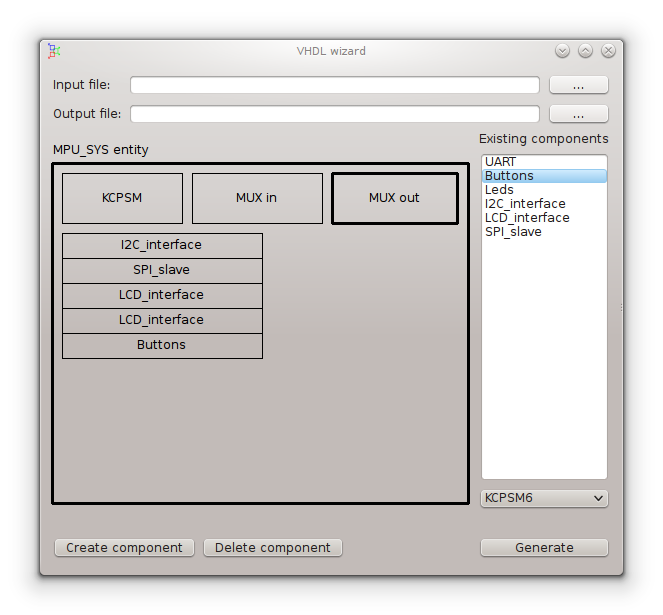
\includegraphics[width=.5\textwidth]{img/VHDL_wizard.png}
    \caption{VHDL Wizard}
\end{figure}

\subsubsection{Purpose of this tool}
    This tool is can be used for easier setting-up of connections between your PicoBlaze implementation and the other parts of your VHDL design. It can help you when you do not want spend too much time writing peripheral logic for PicoBlaze and your VHDL components. This tool automatically takes port addresses from your symbol table file (generated by assembler) and generates corresponding port constants and input/output multiplexers. Final output of this tool is a VHDL entity containing your custom defined components, port constants, all necessary signals/constants, and declaration of KCPSM design.

\subsubsection{Main window}
    \begin{description}
        \item [Input file]
            VHDL wizard reads a symbol table file and extracts all symbols defined with PORT, PORTIN, and PORTOUT directives. Select path to your symbol table (.stbl) file generated after the compilation of you source code. Please make sure that you have enabled generation of the symbol table file (Project->Configure->Compiler->Options->Symbol table).
        \item [Output file]
            The resulting VHDL file.
        \item [MPU\_SYS entity]
            General overview of your VHDL entity. Each box represents one VHDL component, there are always three boxes by default: KCPSM Component, Input Demultiplexer, and Output Multiplexer. You can click to every one of them for detailed information. When you create or add some custom defined components, they will be shown here.
        \item [Existing components]
            This list contains all your previously defined components. For example: let's say you have a UART receiver in your design then create your custom component named UART and define its ports and generic attributes. The newly created component will appear here and you can add it to your entity later.
        \item [KCPSM combobox]
            You can select KCPSM version which you are using in your design, it changes the declaration and instantiation of PicoBlaze in the generated VHDL file. By default it is KCPSM6.
        \item [Create component button]
            This button will open create component dialog where you can define your new component. See the next section "Create component dialog".
        \item [Delete component button]
            This button removes one component from your MPU\_SYS entity.
        \item [Generate]
            If you have your input and output file selected, this button will trigger generation of the VHDL file.
    \end{description}

\subsubsection{Create component dialog}
    You can define your custom component and add it to the generated entity or save it for later usage. You can \textbf{remove} or \textbf{edit} existing components by right-clicking on them in the field "Existing components".

    \begin{figure}[h]
        \centering
        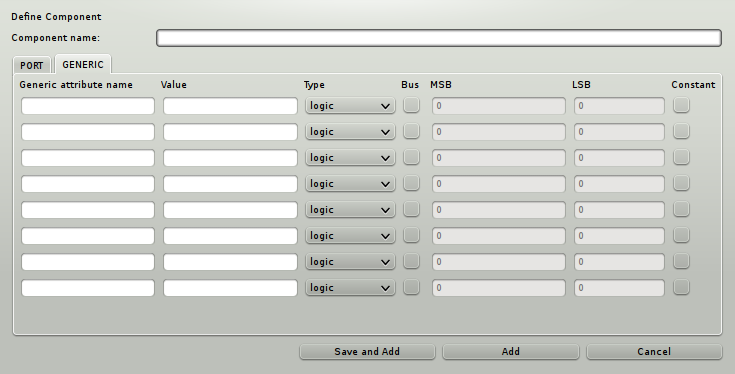
\includegraphics[width=.7\textwidth]{img/VHDL_create_generic.png}
        \caption{Generic parameters of custom component}
    \end{figure}

    \begin{figure}[h]
        \centering
        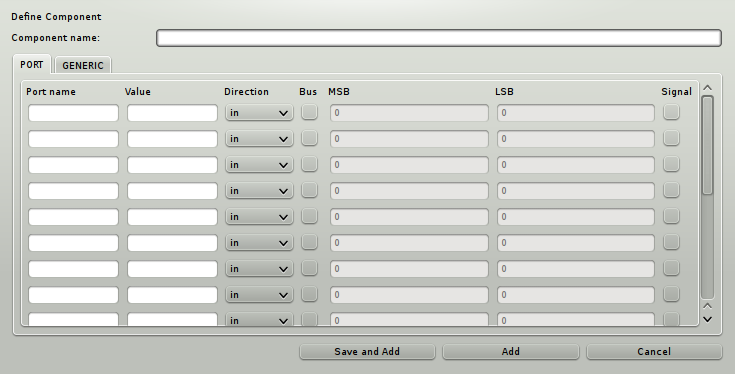
\includegraphics[width=.7\textwidth]{img/VHDL_create_component.png}
        \caption{VHDL port parameters}
    \end{figure}

    \begin{description}
        \item [Component name]
            Name of your custom component.
        \item[Tab PORT]
            Port tab lets you define component ports.
            \begin{description}
                \item[Port name]
                    Name of every port. Names (or identifiers) may consist of letters, numbers, and underscore.
                \item [Value]
                    You can set the initial value. Leaving this field empty means no initial value is needed.
                \item [Direction]
                    Direction in port tab can be IN, OUT or INOUT.
                \item [Bus check-box]
                    Telling generator, that this port is bus. Checking this will enable MSB(most significant bit) and LSB(least significant bit) field, which represents width of your bus.
                \item [Signal check-box]
                    If checked, generator will insert this port declared as signal in VHDL template.
            \end{description}
        \item[Tab GENERIC]
            Port tab lets you define generic attributes of defined component.
            \begin{description}
                \item[Port name]
                    Name of every generic attribute. Names (or identifiers) may consist of letters, numbers, and underscore.
                \item [Value]
                    You can set the initial value. Leaving this field empty means no initial value is needed.
                \item [Type]
                    Defines type of your generic attribute. Logic means zero or one. Logic vector is a bus, defined with MSB and LSB numbers.
                    Integer can be number defined in range from -2147483648 to +2147483647. Positive is RANGE 1 TO integer’HIGH. Natural is in RANGE 0 TO integer’HIGH.
                \item [Bus check-box]
                    Telling generator, that this port is bus. Checking this will enable MSB(most significant bit) and LSB(least significant bit) field, which represents width
                    of your bus. This check box in generic tab makes sense only for logic vector type of attribute.
                \item [Constant check-box]
                    If checked, generator will insert this attribute declared as constant in VHDL template.
            \end{description}
        \item [Save and add button]
            Component will be added to MPU\_SYS entity and saved for later usage. Component name will appear in list "Existing components" and can be edited or added to current entity any time.
        \item [Add button]
            This button will add component to the current entity only once.
        \item [Generate]
            If you have your input and output file selected. This button will trigger generation of VHDL template.\\
    \end{description}
